%%%%%
%%Title: HiPi+Bus V0.2 Chapter 4 Section 7
%%Creator: Ando Ki
%%CreationDate: April 1992
%%FileName: sec7
%%RelatedFile: ch4
%%%%%
\section{중재 인터럽트 1}
중재 인터럽트 1(arbitration interrupt 1)은 다중 프로세서 환경의 효과적인
인터럽트 분배를 구현하기 위해 필요한
인터럽트 전송 방법의 한 형태이다. 이 방법은 인터럽트의 동적인 분배를 실현할 수 있으며,
분배 과정에서 프로세서의 불필요한 Context Switching를 막을 수 있도록 구현되어 있다.
다중 프로세서 운영 체제 환경에서 입출력의 제어와 프로세서 사이의 대화 수단 등으로 사용할 수 있다. \\
중재 인터럽트 1은 지정 인터럽트와는 달리 처리기를 지정하지 않고(프로세서의 모임만 지정),
한개 이상의 처리기에 인터럽트를 동시에 전달한 후, 처리기들 끼리 중재를 하여
인터럽트를 접수할 처리기를 하나만 선정하도록 한다.
중재 과정에서 처리기 들은 현재 자신의 상태(상위 프로세서 등의 상태 포함)에 따라
우선 순위 경쟁을 하게 되는데, 그 순간에 인터럽트를 처리하기에 가장 적절한 것이 선정된다. \\
중재 인터럽트 1도 다른 인터럽트와 같이 인터럽트 버스 사용에 관한 중재 주기가 
끝난 바로 다음 주기부터 요청기에 의하여 시작되고, 22 개의 단계로 구성된다.
첫 단계는 인터럽트 종류, 벡터의 종류 그리고 처리기의 모임을 지정하는 정보를 전송하고,
단계1에서는 단계0에서 전달된 정보를 처리기들이 처리하는 시간이고,
단계2부터 단계16까지는 처리기들 사이의 중재가 진행된다.,
단계17에서는 요청기의 어드레스를 전송하고, 단계18과 단계19에서는 16 비트의
벡터를 전송하고, 단계20에서는 응답기가 이제까지 받은 정보에 대한 점검을 하고,
끝으로 단계21에 처리기는 요청기로 받은 인터럽트에 대한 응답을 보낸다. \\
{\tt <}표~\ref{table:arb-int}{\tt >}는 중재 인터럽트 1의
각 단계 별 전송되는 정보와 방향등을 나타내고 있다.
표에서 처리기에 복수로 표현된 것은 여러개의 처리기가 동작에 참여한다는 것을 의미한다.
%\documentstyle[a4]{hbook}
%\begin{document}
%
\begin{table}[htbp]
\caption{중재 인터럽트 1의 단계별 전송 정보}\label{table:arb-int}
   \begin{center}
   \begin{tabular}{|l|l|l|l|} \hline
	phase & transfer information & from & to \\
\hline \hline
	-5 & Interrupt Class + slot id + id in slot & IR & IR's \\
	-4 & Interrupt Class + slot id + id in slot & IR & IR's \\
	-3 & Interrupt Class + slot id + id in slot & IR & IR's \\
	-2 & Interrupt Class + slot id + id in slot & IR & IR's \\
	-1 & Interrupt Class + slot id + id in slot & IR & IR's \\ \hline
	0 & Interrupt Class + Type + Destination Group ID & IR & IH's \\ \hline
	1 & dummy                                         & - & - \\ \hline
	2 & invers num. of Interrupts in Handler & IH's & IH's \\
	3 & invers num. of Interrupts in Handler & IH's & IH's \\
	4 & invers num. of Interrupts in Handler & IH's & IH's \\
	5 & invers num. of Interrupts in Handler & IH's & IH's \\
	6 & invers num. of Interrupts in Handler & IH's & IH's \\ \hline
	7 & invers Priority of Process & IH's & IH's \\
	8 & invers Priority of Process & IH's & IH's \\
	9 & invers Priority of Process & IH's & IH's \\
	10 & invers Priority of Process & IH's & IH's \\
	11 & invers Priority of Process & IH's & IH's \\ \hline
	12 & Slot Address of Handler & IH's & IH's \\
	13 & Slot Address of Handler & IH's & IH's \\
	14 & Slot Address of Handler & IH's & IH's \\
	15 & Slot Address of Handler & IH's & IH's \\
	16 & Slot Address of Handler & IH's & IH's \\ \hline
	17 & Source Address & IR & IH \\ \hline
	18 & Vector 1 & IR & IH \\ \hline
	19 & Vector 0 & IR & IH \\ \hline
	20 & dummy & - & - \\ \hline
	21 & Acknowledge & IH & IR \\ \hline
   \end{tabular}
   \end{center}
\end{table}
%
%\end{document}

그리고 {\tt <}그림~\ref{figure:arb1-int}{\tt >}는 실제
인터럽트 버스상에서의 동작을 보이고 있다.
%
\begin{figure}[htb]
    \centerline{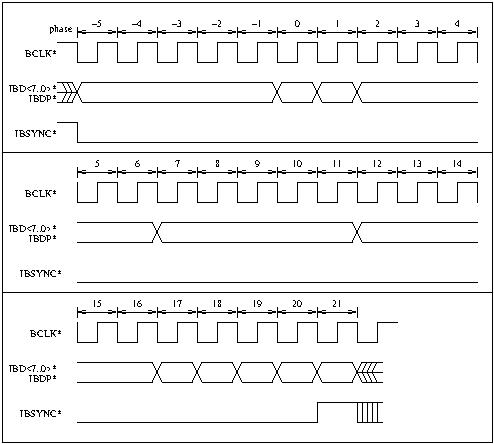
\includegraphics{ch4/FIG/arb1-int.jpg}}
   \caption{중재인터럽트1의 버스 동작}\label{figure:arb1-int}
\end{figure}
%
%
\subsection*{중재 인터럽트 1 - 단계 -5 -- 단계 -1}
인터럽트 버스를 사용하기에 앞서 수행하는 중재 주기이다.
인터럽트 요청기는 현재 진행중인 단계가 중재 인터럽트를 보내기에 앞서 수행하는 중재 주기임을
알리기 위해 IBSYNC* 신호를 구동한다.
%
\subsection*{중재 인터럽트 1 - 단계 0}
인터럽트 요청기는 현재 중재 인터럽트 전송이 진행되고 있음을 알리기 위해 IBSYNC* 신호를 구동한다.
단계 0(phase 0)에서 전송되는 정보는
{\tt <}표~\ref{table:arb-int-p0}{\tt >}과 같이 인터럽트 종류 (Class), 
벡터의 형태 (Type)와 처리기들의 모임 주소 (Group ID)가 전송된다. 
인터럽트 종류 필드는 중재 인터럽트 1을 나타내는 ``2''가 전송된다.
%\documentstyle[a4]{hbook}
%\begin{document}
%
\begin{table}[htbp]
\caption{중재 인터럽트 1 - 단계 0에서 전송되는 정보}\label{table:arb-int-p0}
   \begin{center}
   \begin{tabular}{|l|l|} \hline
	bit field & information \\
\hline \hline
	7, 6 & 2 \\ \hline
	5, 4 & vector type \\ \hline
	3, 2, 1, 0 & group id \\
\hline
   \end{tabular}
   \end{center}
\end{table}
%
%\end{document}

벡터의 종류에 관한 정보가 단계 0에서 전송되는 것이 지정 인터럽트와 다른점으로 볼 수 있다.
벡터의 종류를 단계 0에서 전송하는 이유는 단계 2에서 16까지 진행되는 중재에서
이 정보가 필요하기 때문이다.
중재 인터럽트에서 사용할 수 있는 형태는 {\tt <}표~\ref{table:arb-int-vec}{\tt >}와 같다.
%\documentstyle[a4]{hbook}
%\begin{document}
%
\begin{table}[htbp]
\caption{중재 인터럽트 1의 벡터 형태}\label{table:arb-int-vec}
   \begin{center}
   \begin{tabular}{|l|l|l|} \hline
	type & name & description \\
\hline \hline
	0 & Q-type & queue interrupt \\
	1 & N-type & notify interrupt \\
	2 & AI-1 type-2 & {\it reserved} \\
	3 & AI-1 type-3 & {\it reserved} \\
\hline
   \end{tabular}
   \end{center}
\end{table}
%
%\end{document}

중재 인터럽트의 주된 이용은 다중 처리 운영 체제가 동작하는데 있어서 프로세서들 사이의
동적인 인터럽트의 분배를 위한 것이다. 따라서 벡터 종류도 그와 같은 응용과 밀접한
관계를 갖고 있다. 
\begin{itemize}
	\item N-Type은 notify라는 말이 의미하는 바와 같이 임의의 순간에 발생한 어떤 사건을
	처리기로 통고하는 의미를 지닌다. 따라서 그 인터럽트는 시간과 관계를 갖고 있기 때문에
	시간이 지나면 그 의미를 상실할 수 있다.
	또한 인터럽트가 처리되지 않은 상태에서 또 다시 그 인터럽트가 발생할 경우는
	이와 같은 인터럽트에 해당되는 것은 \ref{section:n-type}에서 설명한 바와 같다.
	\item Q-Type은 한번 전달된 인터럽트는 처리될 때까지 Queue에 저장된다.
	즉 한번 발생된 인터럽트는 무시될 수 없고, 처리가 지연될 수 있으나 무시될 수 없다.
	입출력 인터럽트와 같이 대부분의 인터럽트가 이 형태에 해당된다.
	따라서 인터럽트를 저장할 장소가 없어 인터럽트가 지연될 경우에 새로운 인터럽트가 도착하면
	요청기로 버퍼에 여유가 없음을 알린다.
	처리기에 Queue(FIFO Buffer)를 사용하여 구현하지 않는 경우(오직 한개의 인터럽트만
	저장할 수 있음)는 요청기에서 재시도(retry)를 통해서 Queue의 기능을 대신할 수 있다.
\end{itemize}
%
모임 주소(Group ID)는 처리기들과 연결된 프로세서들을 서로 기능적으로
분류한 주소를 말한다. 본 인터럽트 버스에서는 {\tt <}표~\ref{table:group-id}{\tt >}와 같이
4 종류의 모임을 갖을 수 있고 현재 정의된 주소는 3 개이다.
모임 주소는 비트별로 할당되어 따라서 동시에 2 개 이상의 모임을 선택할 수 있다.
{\tt <}표~\ref{table:group-id}{\tt >}는
모임 주소 각 비트가 지정하는 처리기(해당 프로세서)를 보여 주고 있다.
%\documentstyle[a4]{hbook}
%\begin{document}
%
\begin{table}[htbp]
\caption{중재 인터럽트 1의 모임 주소 각 비트별 의미}\label{table:group-id}
   \begin{center}
   \begin{tabular}{|l|l|} \hline
	group id bit field & group name \\
\hline \hline
	bit 3 & system controllers \\
	bit 2 & input-output processors \\
	bit 1 & {\it reserved} \\
	bit 0 & general purpose processors \\
\hline
   \end{tabular}
   \end{center}
\end{table}
%
%\end{document}

\begin{itemize}
	\item 비트3은 시스템 콘트롤러 그룹을 지정하며, 시스템 제어를 할 수 있는 처리기들이 지정된다.
	\item 비트2는 입출력 처리를 맡고 있는 처리기들이 지정되며, 입출력 프로세서와 시스템 콘트롤러 안에
	입출력 처리 기능을 수행하는 부분에 해당되는 처리기가 지정된다.
	\item 비트0는 일반적인 데이터 처리를 할 수 있는 처리기(프로세서)가 지정된다.
	\item 비트1는 현재 지정되지 않은 것으로 실시간 처리나 그밖의 응용을 위하여 유보하고 있다.
\end{itemize}
각 비트는 어느 조합으로도 동시에 지정이 가능함으로써 3 비트를 동시에 구동하면
시스템 안의 모든 처리기로 중재 인터럽트를 보내게 된다.
%
\subsection*{중재 인터럽트 1 - 단계 1}
인터럽트 요청기는 현재 중재 인터럽트 전송이 진행되고 있음을 알리기 위해 IBSYNC* 신호를 구동한다.
인터럽트 처리기들은 단계 0(phase 0)에서 전송된 정보를 처리한다.
%
\subsection*{중재 인터럽트 1 - 단계 2 --- 단계 6}
인터럽트 요청기는 현재 중재 인터럽트 전송이 진행되고 있음을 알리기 위해 IBSYNC* 신호를 구동한다.
단계 2 (phase 2)부터는 단계 0에서 지정된 처리기들 사이에 수행되는 중재 동작의 첫 단계이다.
처리기들 사이의 중재는 3단계로 구성되는데, {\tt <}표~\ref{table:arb-int}{\tt >}의
단계 2에서 단계 16까지가 해당된다.
지정된 모임 안에 해당되는 처리기들은 각 단계마다 우선 순위 경쟁을 수행하고,
수행한 단계에서 선정된 것들만 계속되는 중재 주기를 수행한다.
결과적으로 단계 16을 마친 후에는 하나의 처리기만 선정되게 된다.
따라서 단계별로 우선 순위가 적용되어 단계 2가 가장 높은 우선 순위 경쟁이 된다. \\
이 단계에서 처리기들이 우선 순위 경쟁을 위해 사용하는 
정보는 처리기 안에 현재 있는 인터럽트 갯수의 역수와 인터럽트 마스크 비트의 
상태
(마스크 되어 있을 경우 0으로 버스에 구동한다) 이다.
%(마스크 되어 있을 경우를
%0으로 함, 즉 가장 높은 우선 순위를 갖는 처리기의 상태는
%모든 비트가 1이 됨)이다. 
이와 같은 중재 정보가 의미하는 것은 마스크가 되어 있지 않을수록, 그리고
처리가 지연되고 있는 인터럽트(Pended Interrupt)가 적은 처리기일수록 
새로운 인터럽트를 접수하는데 있어서 높은 우선 순위를 갖는다는 것이다.
이때 마스크와 인터럽트 갯수는 단계 0에서 지정한 벡터 형태에 관한 것이 된다.
{\tt <}표~\ref{table:arb-int-p2}{\tt >}은 중재 정보로
사용되는 각 데이터의 비트별 할당 상황이다.
%\documentstyle[a4]{hbook}
%\begin{document}
%
\begin{table}[htbp]
\caption{중재 인터럽트 1 - 단계 2에서 사용되는 정보}\label{table:arb-int-p2}
   \begin{center}
   \begin{tabular}{|l|l|} \hline
	bit field & information \\
\hline \hline
	7 & reverse mask bit \\ \hline
	6 & {\it reserved} \\ \hline
	5, 4, 3, 2, 1, 0 & reverse number of interrupts in handler \\
\hline
   \end{tabular}
   \end{center}
\end{table}
%
%\end{document}

%
\subsection*{중재 인터럽트 1 - 단계 7 --- 단계 11}
인터럽트 요청기는 현재 중재 인터럽트 전송이 진행되고 있음을 알리기 위해 IBSYNC* 신호를 구동한다.
단계 7(phase 7)에서는 단계 2의 우선 순위 경쟁에서 이긴 것만 중재를 계속 수행하게 된다.
이 단계에서는 현재 각 처리기에 관련된 프로세서가 수행하고 있는 작업의 우선 순위
(작업의 우선 순위는 운영체제에서 정의한 관리 단위의 수행상 경중을 말함.
UNIX의 경우는 process priority가 이에 해당됨)를 사용하여 중재를 한다.
따라서 새로운 작업을 시작할 때(Context Switching)나 작업의 우선 순위가 변화할 때는
그 우선 순위(Process Priority)를 인터럽트 처리기에 알려주어야 한다.
처리기가 사용할 수 있는 있는 우선 순위는 최대 8 비트이다.
높은 우선 순위를 갖는 작업을 처리하고 있는 프로세서일 경우 이 단계에서 출력되는 정보는
적은 값이 된다.
%\documentstyle[a4]{hbook}
%\begin{document}
%
\begin{table}[htbp]
\caption{중재 인터럽트 1 - 단계 7에서 사용되는 정보}\label{table:arb-int-p7}
   \begin{center}
   \begin{tabular}{|l|l|} \hline
	bit field & information \\
\hline \hline
	7, 6, 5, 4, 3, 2, 1, 0 & inverse priority of process \\
\hline
   \end{tabular}
   \end{center}
\end{table}
%
%\end{document}

%
\subsection*{중재 인터럽트 1 - 단계 12 --- 단계 16}
인터럽트 요청기는 현재 중재 인터럽트 전송이 진행되고 있음을 알리기 위해 IBSYNC* 신호를 구동한다.
단계 12에서도 앞에서와 같이 단계 7까지 우선 순위 경쟁에서 이긴 것들 사이에서만 수행한다.
이 단계에서 사용하는 경쟁 정보는 그 처리기가 현재 위치하는 슬롯 어드레스를 이용한다.
따라서 단계 7까지는 2 개 이상의 처리기가 우선 순위 경쟁에서 이길 수 있으나, 
이 과정을 마치고 나면 항상 1 개의 처리기만이 선정되게 된다.
각 슬롯 어드레스에 대한 위치 배정은 {\tt <}표~\ref{table:arb-int-p12}{\tt >}과 같다.
%\documentstyle[a4]{hbook}
%\begin{document}
%
\begin{table}[htbp]
\caption{중재 인터럽트 1 - 단계 12에서 사용되는 정보}\label{table:arb-int-p12}
   \begin{center}
   \begin{tabular}{|l|l|} \hline
	bit field & information \\
\hline \hline
	7, 6 & 0 \\
	5, 4, 3, 2 & slot id \\
	1, 0 & id in slot \\
\hline
   \end{tabular}
   \end{center}
\end{table}
%
%\end{document}

%
\subsection*{중재 인터럽트 1 - 단계 17}
인터럽트 요청기는 현재 중재 인터럽트 전송이 진행되고 있음을 알리기 위해 IBSYNC* 신호를 구동한다.
이 단계에서는 요청기가 선정된 하나의 처리기로 자신의 주소를 전송한다.
전송되는 정보의 각 비트별 할당은 지정 인터럽트의 단계 1과 같은데,
단지 비트 6과 7을 사용하지 않은 점이 다르다. 이단계에서 사용하는 정보는
{\tt <}표~\ref{table:arb-int-p17}{\tt >}과 같다.
%\documentstyle[a4]{hbook}
%\begin{document}
%
\begin{table}[htbp]
\caption{중재 인터럽트 1 - 단계 17에서 전송되는 정보}\label{table:arb-int-p17}
   \begin{center}
   \begin{tabular}{|l|l|} \hline
	bit field & information \\
\hline \hline
	7, 6 & 0 \\
	5, 4, 3, 2 & slot id \\
	1, 0 & id in slot \\
\hline
   \end{tabular}
   \end{center}
\end{table}
%
%\end{document}

%
\subsection*{중재 인터럽트 1 - 단계 18}
인터럽트 요청기는 현재 중재 인터럽트 전송이 진행되고 있음을 알리기 위해 IBSYNC* 신호를 구동한다.
단계 18에서는 요청기가 처리기로 16 비트의 인터럽트 벡터 중 상위 8 비트를 전송한다.
인터럽트 벡터의 의미는 \ref{section:vector-type}에서 설명한 바와 동일하다.
%\documentstyle[a4]{hbook}
%\begin{document}
%
\begin{table}[htbp]
\caption{중재 인터럽트 1 - 단계 18에서 전송되는 정보}\label{table:arb-int-p18}
   \begin{center}
   \begin{tabular}{|l|l|} \hline
	bit field & information \\
\hline \hline
	7, 6, 5, 4, 3, 2, 1, 0 & most significant byte of interrupt vector \\
\hline
   \end{tabular}
   \end{center}
\end{table}
%
%\end{document}

%
\subsection*{중재 인터럽트 1 - 단계 19}
인터럽트 요청기는 현재 중재 인터럽트 전송이 진행되고 있음을 알리기 위해 IBSYNC* 신호를 구동한다.
단계 19에서는 요청기가 처리기로 16 비트의 인터럽트 벡터 중 하위 8 비트를 전송한다.
인터럽트 벡터의 의미는 \ref{section:vector-type}에서 설명한 바와 동일하다.
%\documentstyle[a4]{hbook}
%\begin{document}
%
\begin{table}[htbp]
\caption{중재 인터럽트 1 - 단계 19에서 전송되는 정보}\label{table:arb-int-p19}
   \begin{center}
   \begin{tabular}{|l|l|} \hline
	bit field & information \\
\hline \hline
	7, 6, 5, 4, 3, 2, 1, 0 & lest significant byte of interrupt vector \\
\hline
   \end{tabular}
   \end{center}
\end{table}
%
%\end{document}

%
\subsection*{중재 인터럽트 1 - 단계 20}
인터럽트 요청기는 현재 중재 인터럽트 전송이 진행되고 있음을 알리기 위해 IBSYNC* 신호를 구동한다.
인터럽트 요청기는 이제까지 받은 정보에 대해 점검하고 다음 단계에 사용할 응답을 준비한다.
%
\subsection*{중재 인터럽트 1 - 단계 21}
인터럽트 요청기는 현재 진행 중인 단계가 중재 인터럽트의 마지막임을 알리기 위해 이제까지
구동하고 있던 IBSYNC* 신호를 걷어낸다.
단계 7에서는 인터럽트 처리기가 인터럽트를 보낸 요청기로 응답을 보내는 단계이다.
이 단계에서 전송되는 신호의 의미는 지정 인터럽트의 경우와 동일하며,
{\tt <}표~\ref{table:dir-int-p3}{\tt >}과 같다.
%%
